\documentclass[12pt,a4paper]{article}

\usepackage[a4paper,margin=1in]{geometry}
\usepackage{graphicx}
\usepackage{booktabs}
\usepackage{amsmath,amssymb}
\usepackage{float}
\usepackage{hyperref}
\usepackage{xcolor}
\usepackage{listings}
\usepackage{enumitem}
\usepackage{fancyhdr}
\usepackage{longtable}

\hypersetup{colorlinks=true,linkcolor=blue,urlcolor=blue}

\pagestyle{fancy}
\fancyhf{}
\lhead{ICS1512}
\rhead{Machine Learning Algorithms Laboratory}
\cfoot{\thepage}

\lstset{
language=Python,
basicstyle=\ttfamily\small,
numbers=left,
frame=single,
breaklines=true,
showstringspaces=false
}

\begin{document}

\begin{tabular}{|p{4cm}|p{11cm}|}
\hline
Experiment No. & 5 \\ \hline
Experiment Title & Decision Tree and Random Forest: A Comparative Classification Study \\ \hline
Student Name & Sathiya Priyan \\ \hline
Register Number & 3122247001058 \\ \hline
Faculty & Dr. Poreddy Ajay Kumar Reddy \\ \hline
Submission Date & August 16, 2026\\ \hline
\end{tabular}

\section{Objective}
\begin{itemize}[nosep]
\item To implement a Decision Tree classifier.
\item To extend the Decision Tree approach into a Random Forest ensemble model.
\item To study the impact of hyperparameters on overfitting and generalization.
\item To select optimal hyperparameters using 5-Fold Cross-Validation.
\item To compare single-tree and ensemble-tree models.
\end{itemize}

\section{Problem Statement}
Given 30 numerical features computed from digitized images of breast mass cell nuclei, the task is to classify each sample as \textbf{Malignant} or \textbf{Benign}. A single Decision Tree classifier is first trained and tuned, after which a Random Forest ensemble is trained and tuned in the same manner. The two models are then compared using standard classification metrics, ROC-AUC, and 5-fold cross-validation, in order to evaluate whether the ensemble approach improves generalization over a single tree.

\section{Dataset Description}
\begin{longtable}{|p{6cm}|p{8cm}|}
\hline
Dataset Name & Wisconsin Diagnostic Breast Cancer Dataset \\ \hline
Dataset Source & \texttt{sklearn.datasets.load\_breast\_cancer} \\ \hline
Number of Samples & 569 \\ \hline
Number of Features & 30 numerical attributes \\ \hline
Number of Classes & 2 (Malignant, Benign) \\ \hline
Missing Values & None (verified using \texttt{df.isnull().sum()}) \\ \hline
Train-Test Split & 80\% train (455 samples) / 20\% test (114 samples), stratified, \texttt{random\_state=42} \\ \hline
\end{longtable}

The target variable is encoded numerically as \texttt{0 = Malignant} and \texttt{1 = Benign}, matching the default encoding of the scikit-learn dataset. This mapping was explicitly verified in the notebook and used to create a readable \texttt{diagnosis} column for analysis.

\vspace{0.2cm}
A brief statistical summary of a few representative features (from \texttt{df.describe()}) is shown below to illustrate the scale differences across features, which motivated checking whether feature scaling would be needed:

\begin{table}[H]
\centering
\caption{Statistical Summary of Selected Features}
\begin{tabular}{lcccc}
\toprule
Feature & Mean & Std. Dev. & Min & Max \\
\midrule
mean radius      & 14.13  & 3.52  & 6.98  & 28.11 \\
mean area        & 654.89 & 351.91 & 143.50 & 2501.00 \\
mean smoothness  & 0.0964 & 0.0141 & 0.0526 & 0.1634 \\
mean concavity   & 0.0888 & 0.0797 & 0.0000 & 0.4268 \\
\bottomrule
\end{tabular}
\end{table}

\section{Exploratory Data Analysis}

\subsection*{Class Distribution}
The dataset contains 357 Benign samples and 212 Malignant samples, indicating a moderate class imbalance (roughly 63\% to 37\%) rather than a severe one.

\begin{figure}[H]
\centering
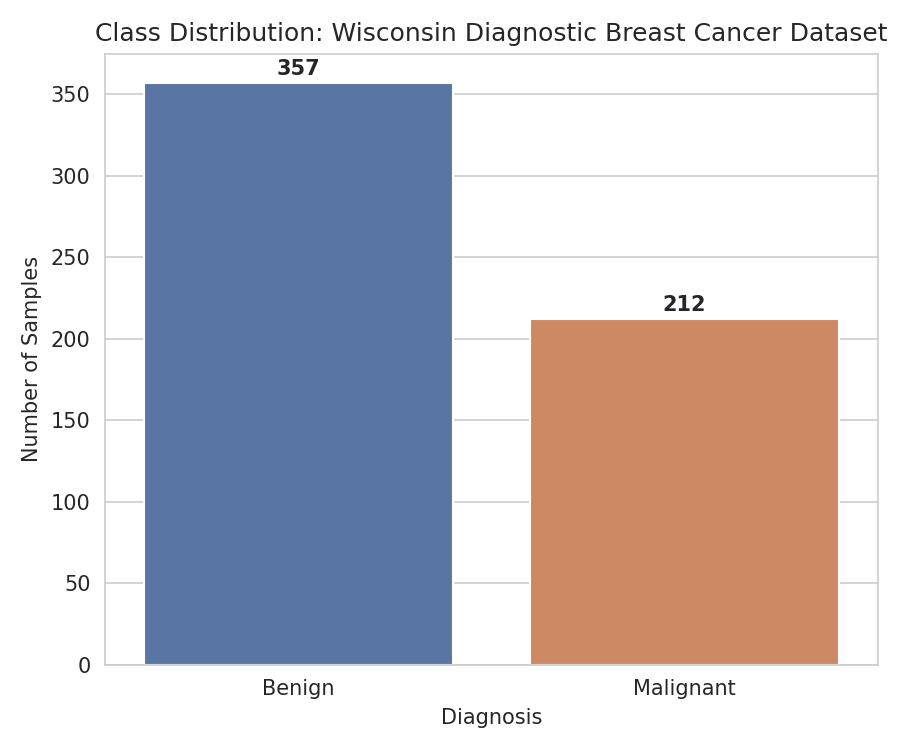
\includegraphics[width=0.62\linewidth]{figures/class_distribution_exp5.png}
\caption{Class distribution of the Wisconsin Diagnostic Breast Cancer Dataset}
\end{figure}

\textbf{Inference:} Benign cases outnumber Malignant cases in the dataset. Because the imbalance is moderate, accuracy remains a reasonably informative metric, but precision, recall and F1-score were also tracked throughout the experiment to avoid a misleading picture of performance on the minority (Malignant) class.

\subsection*{Feature Correlation Analysis}
Since the dataset has 30 features, a full 30$\times$30 correlation heatmap becomes cluttered and hard to read. Instead, the ten most strongly correlated feature pairs (by absolute Pearson correlation) were identified and plotted.

\begin{figure}[H]
\centering
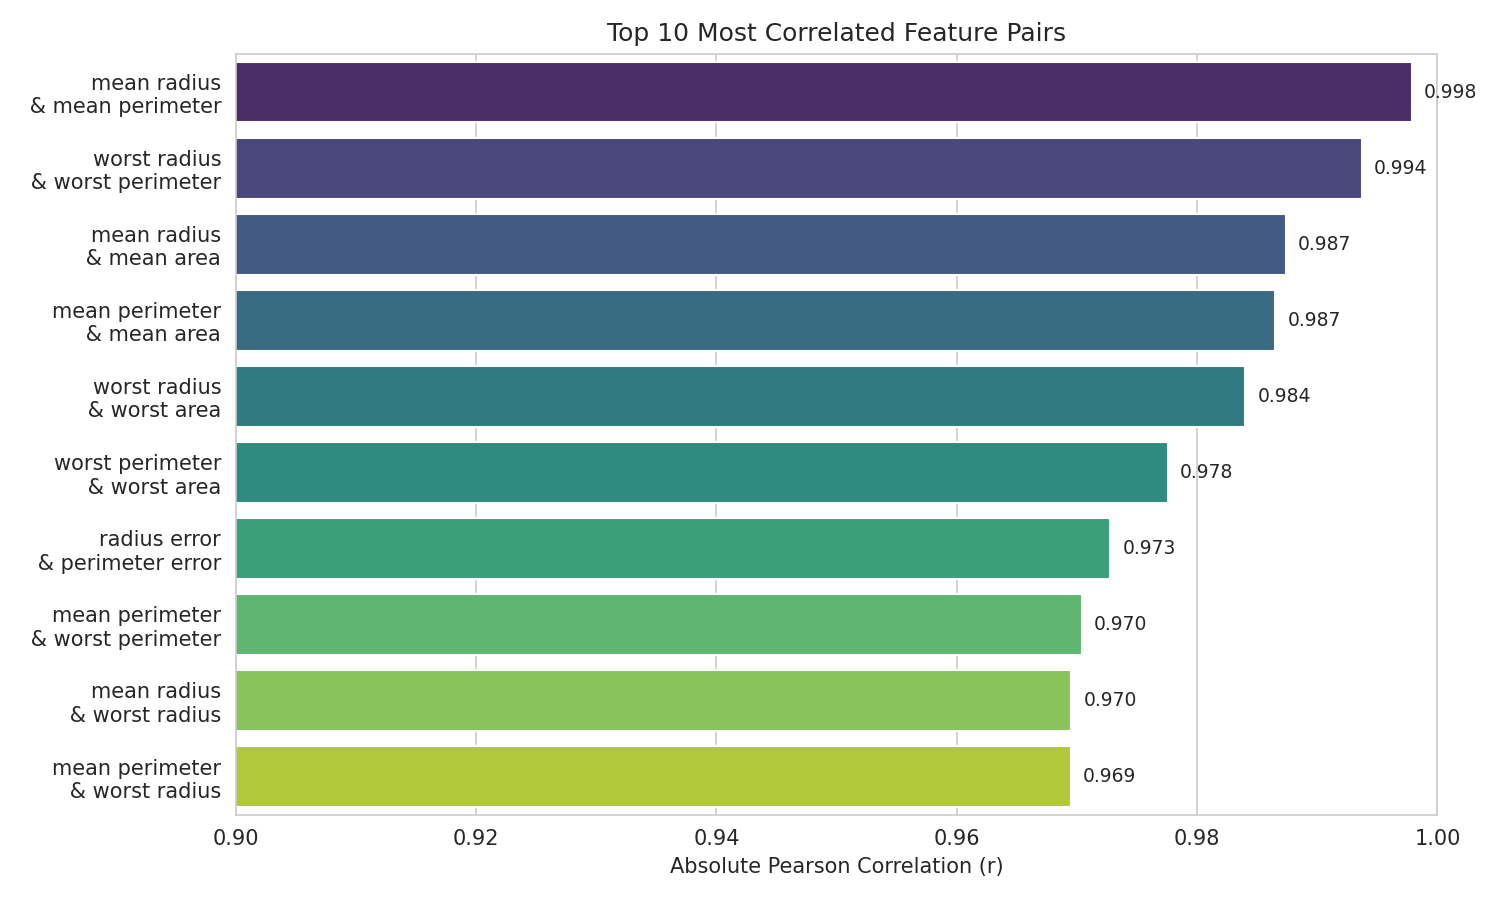
\includegraphics[width=0.88\linewidth]{figures/top_correlations_exp5.png}
\caption{Top 10 most correlated feature pairs}
\end{figure}

\textbf{Inference:} The strongest correlations are between geometrically related measurements, e.g. \texttt{mean radius} and \texttt{mean perimeter} (r = 0.998), and \texttt{worst radius} and \texttt{worst perimeter} (r = 0.994). This is expected since radius, perimeter, and area are mathematically related quantities describing the same physical shape. Such high redundancy suggests that tree-based models, which perform implicit feature selection at each split, are well suited to this dataset since they can naturally ignore redundant correlated features.

\section{Data Preprocessing}
\begin{itemize}[nosep]
\item \textbf{Missing values:} Checked using \texttt{df.isnull().sum()}; no missing values were found, so no imputation was required.
\item \textbf{Encoding:} The target variable was already numerically encoded (0 = Malignant, 1 = Benign) by the source dataset; this mapping was explicitly displayed for clarity.
\item \textbf{Feature scaling:} Not applied. Decision Trees and Random Forests split on individual feature thresholds and are invariant to monotonic feature scaling, so standardization was not necessary.
\item \textbf{Train-test split:} An 80--20 stratified split was used (\texttt{train\_test\_split} with \texttt{test\_size=0.2}, \texttt{random\_state=42}, \texttt{stratify=y}), giving 455 training samples and 114 testing samples while preserving the class ratio in both sets.
\end{itemize}

\section{Machine Learning Algorithm}

\subsection{Decision Tree}
A Decision Tree recursively partitions the feature space by choosing, at each node, the feature and threshold that most reduces impurity (measured using Gini Index or Entropy). Predictions are made by following the decision path from the root to a leaf.

\textbf{Mathematical formulation.} For a node with class proportions $p_i$ ($i = 1, \dots, C$), the two impurity measures used in this experiment are:
\begin{align}
\text{Gini Index} &= 1 - \sum_{i=1}^{C} p_i^2 \\
\text{Entropy} &= -\sum_{i=1}^{C} p_i \log_2(p_i)
\end{align}
At each split, the algorithm chooses the feature and threshold that maximize the impurity reduction (information gain), i.e. the decrease in weighted child-node impurity relative to the parent node.

\begin{itemize}[nosep]
\item \textbf{Advantages:} Easy to interpret, requires no feature scaling, naturally handles non-linear decision boundaries.
\item \textbf{Limitations:} Prone to high variance and overfitting, especially when grown without depth restriction, as a single tree can memorize the training data.
\end{itemize}

\subsection{Random Forest}
Random Forest is an ensemble method that builds many decision trees, each trained on a bootstrap sample of the training data, and further randomizes each split by considering only a random subset of features. Final predictions are made by majority voting across all trees:
\begin{equation}
\hat{y} = \text{mode}\{h_1(x), h_2(x), \dots, h_n(x)\}
\end{equation}
where $h_k(x)$ is the prediction of the $k$-th tree, trained on a bootstrap sample $D_k$ drawn with replacement from the training data, with each split restricted to a random subset of \texttt{max\_features} features.

\begin{itemize}[nosep]
\item \textbf{Advantages:} Reduces variance and overfitting compared to a single tree by averaging over many de-correlated trees; generally improves generalization.
\item \textbf{Limitations:} Less interpretable than a single tree, and more computationally expensive to train and tune due to the larger number of trees and hyperparameters.
\end{itemize}

\section{Experimental Setup}
\begin{tabular}{ll}
\toprule
Python Version & 3.x \\
Scikit-Learn Version & As installed in the notebook environment \\
IDE & Jupyter Notebook \\
Operating System & N/A \\
Hardware & N/A \\
\bottomrule
\end{tabular}

\vspace{0.3cm}
The key libraries used were \texttt{pandas} and \texttt{numpy} for data handling, \texttt{matplotlib} and \texttt{seaborn} for visualization, and \texttt{scikit-learn} for dataset loading (\texttt{load\_breast\_cancer}), model training (\texttt{DecisionTreeClassifier}, \texttt{RandomForestClassifier}), hyperparameter search (\texttt{GridSearchCV}), and evaluation (\texttt{accuracy\_score}, \texttt{precision\_score}, \texttt{recall\_score}, \texttt{f1\_score}, \texttt{confusion\_matrix}, \texttt{classification\_report}, \texttt{roc\_curve}, \texttt{auc}). All random processes (train-test split, tree construction, bootstrap sampling) used \texttt{random\_state=42} for reproducibility.

\section{Hyperparameter Selection}

Both models were tuned using \texttt{GridSearchCV} with 5-fold cross-validation and \texttt{scoring='accuracy'}.

\subsection{Decision Tree}
\begin{tabular}{ll}
\toprule
Parameter & Search Space\\
\midrule
criterion & gini, entropy \\
max\_depth & None, 3, 5, 7, 10 \\
min\_samples\_split & 2, 5, 10 \\
min\_samples\_leaf & 1, 2, 4 \\
\bottomrule
\end{tabular}

\vspace{0.3cm}
\textbf{Best Parameters (GridSearchCV):} criterion = gini, max\_depth = 5, min\_samples\_split = 5, min\_samples\_leaf = 1 \\
\textbf{Best 5-Fold CV Accuracy:} 93.85\%

\vspace{0.3cm}
Table~\ref{tab:dt-tuning} summarizes the average 5-fold CV accuracy and F1-score across criterion and max\_depth combinations (\texttt{min\_samples\_split} and \texttt{min\_samples\_leaf} held at their default values in this summary; the full combination search was performed separately via GridSearchCV above).

\begin{table}[H]
\centering
\caption{Decision Tree Hyperparameter Evaluation using 5-Fold Cross-Validation}
\label{tab:dt-tuning}
\begin{tabular}{llcc}
\toprule
Criterion & Max Depth & Avg CV Accuracy (\%) & Avg CV F1 Score \\
\midrule
gini    & None & 90.99 & 0.9282 \\
gini    & 3    & 92.53 & 0.9416 \\
gini    & 5    & 93.19 & 0.9461 \\
gini    & 7    & 92.09 & 0.9371 \\
gini    & 10   & 90.99 & 0.9282 \\
entropy & None & 93.19 & 0.9450 \\
entropy & 3    & 92.97 & 0.9441 \\
entropy & 5    & 92.53 & 0.9397 \\
entropy & 7    & 93.19 & 0.9450 \\
entropy & 10   & 93.19 & 0.9450 \\
\bottomrule
\end{tabular}
\end{table}

\subsection{Random Forest}
\begin{tabular}{ll}
\toprule
Parameter & Search Space\\
\midrule
n\_estimators & 50, 100, 200 \\
max\_depth & None, 5, 10 \\
max\_features & sqrt, log2 \\
bootstrap & True, False \\
\bottomrule
\end{tabular}

\vspace{0.3cm}
\textbf{Best Parameters (GridSearchCV):} n\_estimators = 100, max\_depth = None, max\_features = log2, bootstrap = False \\
\textbf{Best 5-Fold CV Accuracy:} 96.92\%

\vspace{0.3cm}
Table~\ref{tab:rf-tuning} summarizes the average 5-fold CV accuracy and F1-score for the \texttt{n\_estimators} / \texttt{max\_depth} / \texttt{max\_features} combinations (with \texttt{bootstrap=True}, the scikit-learn default, in this summary). The GridSearchCV run above also explored \texttt{bootstrap=False} and found a marginally better combination overall.

\begin{table}[H]
\centering
\caption{Random Forest Hyperparameter Evaluation using 5-Fold Cross-Validation}
\label{tab:rf-tuning}
\small
\begin{tabular}{lllcc}
\toprule
n\_estimators & Max Depth & Max Features & Avg CV Accuracy (\%) & Avg CV F1 Score \\
\midrule
50  & None & sqrt & 95.16 & 0.9617 \\
50  & None & log2 & 95.38 & 0.9631 \\
50  & 5    & sqrt & 95.16 & 0.9619 \\
50  & 5    & log2 & 95.16 & 0.9616 \\
50  & 10   & sqrt & 95.16 & 0.9617 \\
50  & 10   & log2 & 95.38 & 0.9631 \\
100 & None & sqrt & 95.38 & 0.9634 \\
100 & None & log2 & 95.60 & 0.9648 \\
100 & 5    & sqrt & 94.95 & 0.9601 \\
100 & 5    & log2 & 95.16 & 0.9615 \\
100 & 10   & sqrt & 95.38 & 0.9634 \\
100 & 10   & log2 & 95.60 & 0.9648 \\
200 & None & sqrt & 96.04 & 0.9684 \\
200 & None & log2 & 95.60 & 0.9648 \\
200 & 5    & sqrt & 94.95 & 0.9601 \\
200 & 5    & log2 & 95.38 & 0.9632 \\
200 & 10   & sqrt & 96.04 & 0.9684 \\
200 & 10   & log2 & 95.60 & 0.9648 \\
\bottomrule
\end{tabular}
\end{table}

\section{Results}

\subsection{Baseline Decision Tree}
The baseline Decision Tree (default parameters, \texttt{random\_state=42}) achieved a training accuracy of 100\%, indicating it perfectly memorized the training set.

\begin{tabular}{lc}
\toprule
Metric & Value\\
\midrule
Training Accuracy & 1.0000 \\
Testing Accuracy & 0.9123 \\
Precision & 0.9559 \\
Recall & 0.9028 \\
F1-score & 0.9286 \\
\bottomrule
\end{tabular}

\begin{figure}[H]
\centering
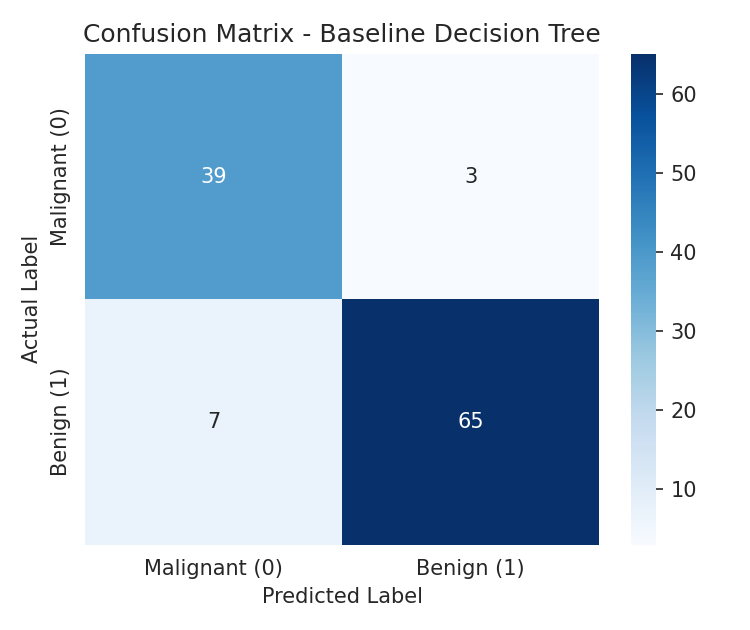
\includegraphics[width=0.52\linewidth]{figures/cm_baseline_dt_exp5.png}
\caption{Confusion Matrix -- Baseline Decision Tree}
\end{figure}

\begin{table}[H]
\centering
\caption{Baseline Decision Tree -- Confusion Matrix Values}
\begin{tabular}{lcc}
\toprule
 & Predicted Malignant (0) & Predicted Benign (1) \\
\midrule
Actual Malignant (0) & 39 & 3 \\
Actual Benign (1)    & 7  & 65 \\
\bottomrule
\end{tabular}
\end{table}

\vspace{0.2cm}
\textbf{Per-class classification report:}
\begin{table}[H]
\centering
\begin{tabular}{lcccc}
\toprule
Class & Precision & Recall & F1-score & Support \\
\midrule
0 (Malignant) & 0.85 & 0.93 & 0.89 & 42 \\
1 (Benign)    & 0.96 & 0.90 & 0.93 & 72 \\
\midrule
Macro avg     & 0.90 & 0.92 & 0.91 & 114 \\
Weighted avg  & 0.92 & 0.91 & 0.91 & 114 \\
\bottomrule
\end{tabular}
\end{table}

\subsection{Tuned Decision Tree}
Using the best parameters found by GridSearchCV (criterion = gini, max\_depth = 5, min\_samples\_split = 5, min\_samples\_leaf = 1):

\begin{tabular}{lc}
\toprule
Metric & Value\\
\midrule
Accuracy & 0.9211 \\
Precision & 0.9565 \\
Recall & 0.9167 \\
F1-score & 0.9362 \\
ROC-AUC & 0.9163 \\
\bottomrule
\end{tabular}

\begin{figure}[H]
\centering
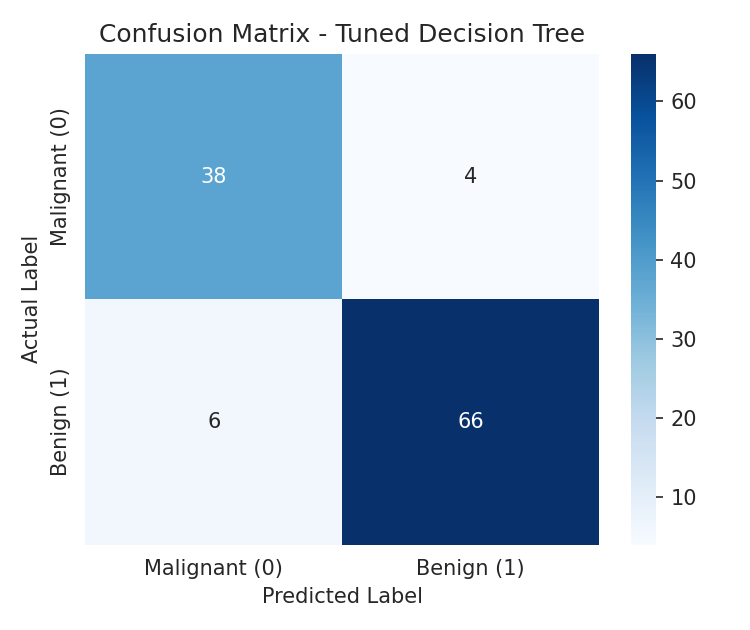
\includegraphics[width=0.52\linewidth]{figures/cm_best_dt_exp5.png}
\caption{Confusion Matrix -- Tuned Decision Tree}
\end{figure}

\begin{table}[H]
\centering
\caption{Tuned Decision Tree -- Confusion Matrix Values}
\begin{tabular}{lcc}
\toprule
 & Predicted Malignant (0) & Predicted Benign (1) \\
\midrule
Actual Malignant (0) & 39 & 3 \\
Actual Benign (1)    & 6  & 66 \\
\bottomrule
\end{tabular}
\end{table}

\vspace{0.2cm}
\textbf{Per-class classification report:}
\begin{table}[H]
\centering
\begin{tabular}{lcccc}
\toprule
Class & Precision & Recall & F1-score & Support \\
\midrule
0 (Malignant) & 0.87 & 0.93 & 0.90 & 42 \\
1 (Benign)    & 0.96 & 0.92 & 0.94 & 72 \\
\midrule
Macro avg     & 0.91 & 0.92 & 0.92 & 114 \\
Weighted avg  & 0.92 & 0.92 & 0.92 & 114 \\
\bottomrule
\end{tabular}
\end{table}

\textbf{Inference:} Tuning improved test accuracy from 91.23\% (baseline) to 92.11\% and reduced the gap between training and testing performance, showing that restricting tree depth via cross-validated tuning reduces overfitting compared to the fully grown baseline tree. The per-class report shows the improvement is concentrated in the Benign class recall (0.90 to 0.92), while Malignant-class recall stayed at 0.93 in both cases.

\subsection{Baseline Random Forest}
\begin{tabular}{lc}
\toprule
Metric & Value\\
\midrule
Accuracy & 0.9561 \\
Precision & 0.9589 \\
Recall & 0.9722 \\
F1-score & 0.9655 \\
\bottomrule
\end{tabular}

\begin{figure}[H]
\centering
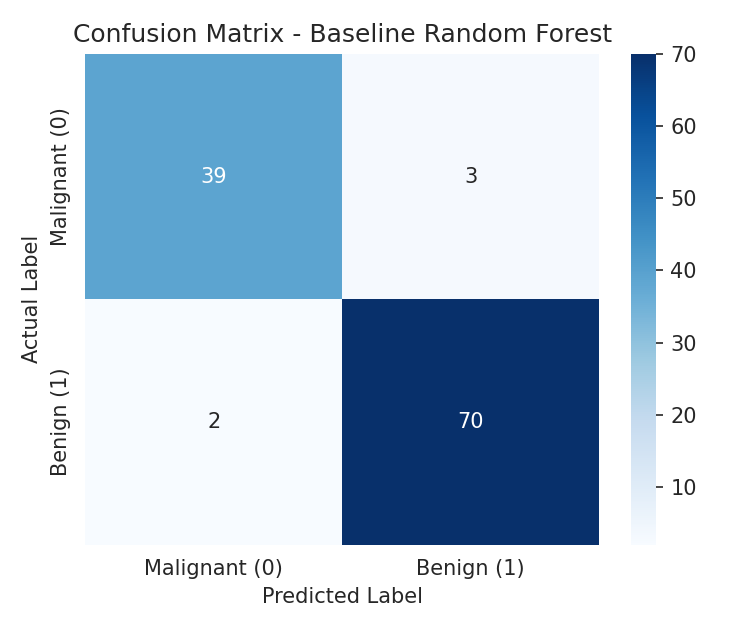
\includegraphics[width=0.52\linewidth]{figures/cm_baseline_rf_exp5.png}
\caption{Confusion Matrix -- Baseline Random Forest}
\end{figure}

\begin{table}[H]
\centering
\caption{Baseline Random Forest -- Confusion Matrix Values}
\begin{tabular}{lcc}
\toprule
 & Predicted Malignant (0) & Predicted Benign (1) \\
\midrule
Actual Malignant (0) & 39 & 3 \\
Actual Benign (1)    & 2  & 70 \\
\bottomrule
\end{tabular}
\end{table}

\vspace{0.2cm}
\textbf{Per-class classification report:}
\begin{table}[H]
\centering
\begin{tabular}{lcccc}
\toprule
Class & Precision & Recall & F1-score & Support \\
\midrule
0 (Malignant) & 0.95 & 0.93 & 0.94 & 42 \\
1 (Benign)    & 0.96 & 0.97 & 0.97 & 72 \\
\midrule
Macro avg     & 0.96 & 0.95 & 0.95 & 114 \\
Weighted avg  & 0.96 & 0.96 & 0.96 & 114 \\
\bottomrule
\end{tabular}
\end{table}

\subsection{Tuned Random Forest}
Using the best parameters found by GridSearchCV (n\_estimators = 100, max\_depth = None, max\_features = log2, bootstrap = False):

\begin{tabular}{lc}
\toprule
Metric & Value\\
\midrule
Accuracy & 0.9561 \\
Precision & 0.9589 \\
Recall & 0.9722 \\
F1-score & 0.9655 \\
ROC-AUC & 0.9944 \\
\bottomrule
\end{tabular}

\begin{figure}[H]
\centering
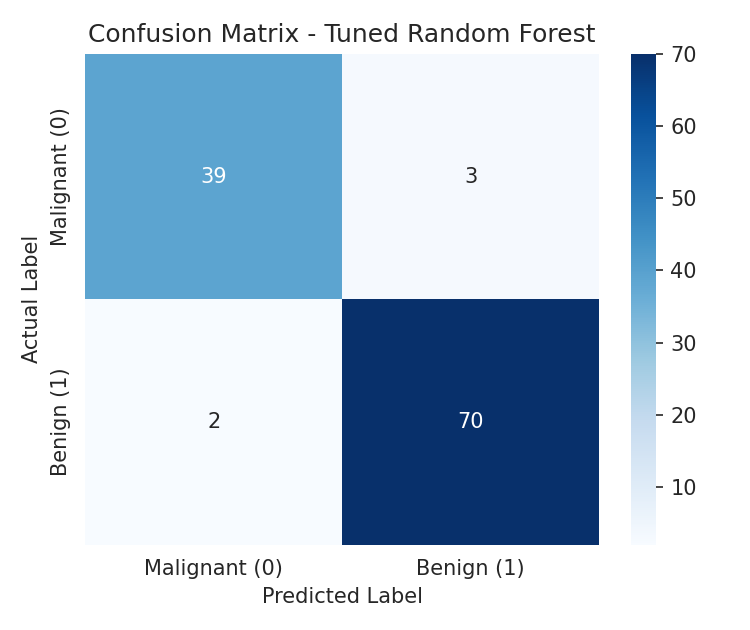
\includegraphics[width=0.52\linewidth]{figures/cm_best_rf_exp5.png}
\caption{Confusion Matrix -- Tuned Random Forest}
\end{figure}

\begin{table}[H]
\centering
\caption{Tuned Random Forest -- Confusion Matrix Values}
\begin{tabular}{lcc}
\toprule
 & Predicted Malignant (0) & Predicted Benign (1) \\
\midrule
Actual Malignant (0) & 39 & 3 \\
Actual Benign (1)    & 2  & 70 \\
\bottomrule
\end{tabular}
\end{table}

\vspace{0.2cm}
\textbf{Per-class classification report:}
\begin{table}[H]
\centering
\begin{tabular}{lcccc}
\toprule
Class & Precision & Recall & F1-score & Support \\
\midrule
0 (Malignant) & 0.95 & 0.93 & 0.94 & 42 \\
1 (Benign)    & 0.96 & 0.97 & 0.97 & 72 \\
\midrule
Macro avg     & 0.96 & 0.95 & 0.95 & 114 \\
Weighted avg  & 0.96 & 0.96 & 0.96 & 114 \\
\bottomrule
\end{tabular}
\end{table}

\textbf{Inference:} The tuned Random Forest matched the baseline Random Forest on the test set, both clearly outperforming the Decision Tree on every metric. This indicates that Random Forest is inherently robust to hyperparameter choice on this dataset, unlike the single tree which needed depth restriction to reduce overfitting.

\subsection{ROC Curve and AUC Comparison}
\begin{figure}[H]
\centering
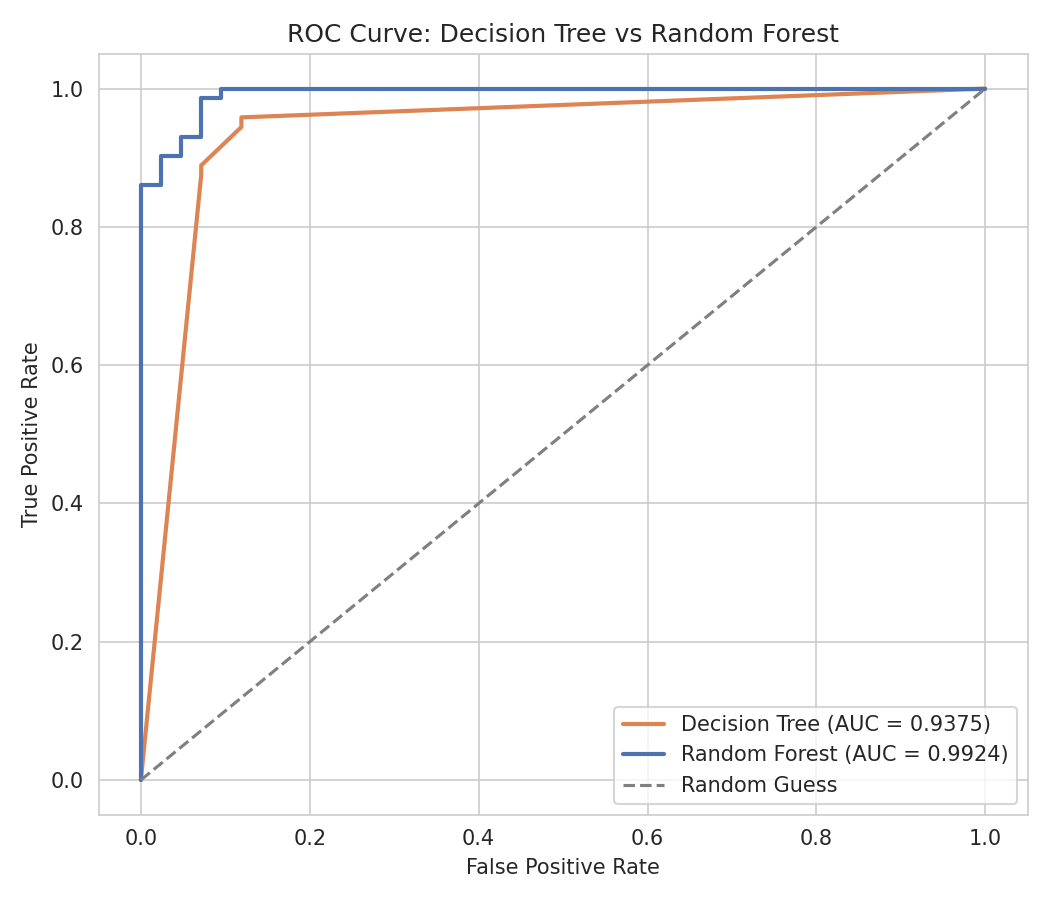
\includegraphics[width=0.68\linewidth]{figures/roc_curve_exp5.png}
\caption{ROC Curve -- Decision Tree vs. Random Forest}
\end{figure}

\textbf{Inference:} The Random Forest achieved an AUC of 0.9944 compared to 0.9163 for the Decision Tree. The Random Forest's ROC curve stays much closer to the top-left corner, showing it separates the Malignant and Benign classes far more reliably across all classification thresholds than the single tree.

\subsection{Model Comparison}
\begin{table}[H]
\centering
\caption{Decision Tree vs. Random Forest -- Test Set Comparison}
\begin{tabular}{lcccccc}
\toprule
Model & Accuracy & Precision & Recall & F1 Score & AUC \\
\midrule
Decision Tree & 0.9211 & 0.9565 & 0.9167 & 0.9362 & 0.9163 \\
Random Forest & 0.9561 & 0.9589 & 0.9722 & 0.9655 & 0.9944 \\
\bottomrule
\end{tabular}
\end{table}

The Random Forest outperforms the Decision Tree on every single metric on the held-out test set.

\subsection{5-Fold Cross-Validation Performance Comparison}
\begin{table}[H]
\centering
\caption{5-Fold Cross-Validation Accuracy Comparison}
\begin{tabular}{lcccccc}
\toprule
Model & Fold 1 & Fold 2 & Fold 3 & Fold 4 & Fold 5 & Average \\
\midrule
Decision Tree & 0.9451 & 0.9451 & 0.9011 & 0.9451 & 0.9560 & 0.9385 \\
Random Forest & 0.9780 & 1.0000 & 0.9341 & 0.9560 & 0.9780 & 0.9692 \\
\bottomrule
\end{tabular}
\end{table}

\textbf{Inference:} The Random Forest achieved a higher accuracy than the Decision Tree in every one of the 5 folds, and a higher average accuracy overall (96.92\% vs 93.85\%). Fold 3 was the weakest fold for both models, suggesting that particular training/validation split was inherently harder, but Random Forest still handled it better than the Decision Tree (93.41\% vs 90.11\%).

\section{Result Visualization}

The key visualizations generated during the experiment are the class distribution plot, the top-10 feature correlation plot, the confusion matrices, and the ROC curve, all presented in the sections above alongside their inferences. Confusion matrices for the baseline models were also generated in the notebook and follow the same pattern as their tuned counterparts, so they are omitted here to keep the report within the page limit.

\section{Discussion}

\subsection{Overview of Results}
Across every stage of the experiment -- baseline models, tuned models, ROC-AUC, and 5-fold cross-validation -- the Random Forest consistently outperformed the single Decision Tree. The gap was largest in ROC-AUC (0.9944 vs 0.9163, a difference of 0.078), moderate in test accuracy (95.61\% vs 92.11\%, a 3.5 point difference), and smallest but still consistent in precision (0.9589 vs 0.9565). This pattern is consistent with the theoretical expectation that ensembling primarily reduces variance-driven errors, which tend to show up more strongly in threshold-sensitive metrics like AUC than in metrics computed at a single fixed threshold like precision.

\subsection{Comparative Analysis}
\textbf{Best-performing classifier:} The Random Forest was the best-performing model overall, outperforming the Decision Tree on test accuracy (95.61\% vs 92.11\%), precision, recall, F1-score, ROC-AUC (0.9944 vs 0.9163), and average 5-fold CV accuracy (96.92\% vs 93.85\%).

\textbf{Effect of hyperparameter tuning:} Decision Tree tuning had a visible effect: the baseline tree overfit the training data completely (100\% training accuracy) while testing at only 91.23\%. Restricting \texttt{max\_depth} to 5 (found via GridSearchCV) improved test accuracy to 92.11\% and brought the CV-estimated performance (93.85\%) closer to the test performance, indicating reduced overfitting. In contrast, Random Forest hyperparameter tuning had almost no effect on the test set, since the baseline and tuned Random Forest produced identical test metrics -- the ensembling process itself was already stabilizing predictions regardless of the exact tree count or feature subset size.

\textbf{Behaviour of SVM kernels:} Not applicable to this experiment, since Experiment 5 covers Decision Tree and Random Forest models only.

\textbf{Bias-variance trade-off:} The baseline Decision Tree illustrates a classic high-variance, low-bias regime: it fits the training data perfectly but generalizes worse to unseen data. Restricting tree depth trades a small amount of bias for a meaningful reduction in variance, improving test performance. The Random Forest reduces variance further still by averaging over many de-correlated trees (via bootstrap sampling and random feature selection), which explains its consistently higher and more stable accuracy across all 5 cross-validation folds and its higher AUC.

\subsection{Observation Questions}

\textbf{1. How does tree depth affect overfitting in Decision Trees?}\\
The baseline Decision Tree, grown without a depth restriction, reached 100\% training accuracy but only 91.23\% test accuracy -- a clear sign of overfitting. In the hyperparameter table (Table~\ref{tab:dt-tuning}), the gini-criterion tree's CV accuracy peaked at \texttt{max\_depth = 5} (93.19\%) and declined again by \texttt{max\_depth = 10} (90.99\%), matching the unrestricted-depth score. This shows that allowing the tree to grow too deep lets it fit noise in the training folds, hurting cross-validated performance, while a moderate depth limit improves generalization. The entropy-criterion tree was comparatively less sensitive to depth, staying between 92.5\% and 93.2\% across all depths tested.

\textbf{2. Which hyperparameter had the greatest impact on performance?}\\
Among the parameters summarized in Table~\ref{tab:dt-tuning}, \texttt{max\_depth} had the most visible impact when using the gini criterion, producing a 2.2 percentage-point spread in CV accuracy (90.99\% to 93.19\%) depending on depth. However, the overall best result from the full GridSearchCV (93.85\% CV accuracy) was obtained only when \texttt{min\_samples\_split} was also set to 5 alongside \texttt{max\_depth = 5}, exceeding every value in the depth-only summary table. This suggests that \texttt{max\_depth} was the single most influential parameter, but its effect was compounded by \texttt{min\_samples\_split}, which further limited node splitting. For Random Forest, \texttt{max\_features} consistently mattered more than \texttt{bootstrap} or \texttt{max\_depth} in the summary table: for a fixed \texttt{n\_estimators}, changing \texttt{max\_features} from \texttt{sqrt} to \texttt{log2} generally matched or improved CV accuracy (e.g. at \texttt{n\_estimators=100}, \texttt{max\_depth=None}: 95.38\% with sqrt vs 95.60\% with log2).

\textbf{3. How does Random Forest improve generalization?}\\
Random Forest builds many trees, each on a bootstrap sample of the training data and each restricted to a random subset of features at every split. This decorrelates the individual trees, so their errors are less likely to coincide, and averaging their predictions through majority voting reduces the overall variance of the model. In this experiment, this is reflected in the Random Forest's higher and more consistent 5-fold CV accuracy (96.92\% average, ranging only from 93.41\% to 100\%) compared to the Decision Tree (93.85\% average, ranging from 90.11\% to 95.60\%), as well as its much higher AUC (0.9944 vs 0.9163), which shows more reliable class separation across all decision thresholds.

\textbf{4. Did ensemble learning always improve performance? Why or why not?}\\
In this experiment, Random Forest outperformed the Decision Tree on every test-set metric and in every one of the 5 cross-validation folds (Table~\ref{tab:dt-tuning} vs Table~\ref{tab:rf-tuning}, and the fold-wise comparison table), so ensembling did consistently improve performance here. This is not a universal guarantee, however: ensemble learning improves performance mainly when the base learners (individual trees) are reasonably accurate but make somewhat independent errors. On a dataset with strongly redundant, well-separated features such as this one, both single trees and forests already perform well, but the forest's variance reduction still gave a measurable and consistent edge. If the base trees were very weak or highly correlated, or if the dataset were simpler still, the improvement from ensembling could be much smaller.

\subsection{Limitations}
The evaluation is based on a single 80--20 train-test split and a single 5-fold cross-validation run with a fixed \texttt{random\_state}, so the reported numbers could shift slightly under a different random seed or split. The hyperparameter search spaces, while covering the parameters required by the assignment, were not exhaustive (e.g. \texttt{max\_depth} values beyond 10 were not tested for the Decision Tree, and \texttt{n\_estimators} beyond 200 was not tested for the Random Forest), so the reported "best" parameters are best only within the explored grid, not globally optimal.

\section{Conclusion}
A Decision Tree and a Random Forest classifier were implemented on the Wisconsin Diagnostic Breast Cancer Dataset and tuned using GridSearchCV with 5-fold cross-validation over the required hyperparameters (\texttt{criterion}, \texttt{max\_depth}, \texttt{min\_samples\_split}, \texttt{min\_samples\_leaf} for the Decision Tree; \texttt{n\_estimators}, \texttt{max\_depth}, \texttt{max\_features}, \texttt{bootstrap} for the Random Forest). The baseline Decision Tree overfit the training data (100\% training accuracy vs 91.23\% test accuracy), and tuning improved its test accuracy to 92.11\% by restricting depth. The Random Forest was more robust to the choice of hyperparameters, with baseline and tuned versions achieving identical test performance (95.61\% accuracy, 0.9655 F1-score, 0.9944 AUC). Across all comparisons -- test-set metrics, ROC-AUC, and all 5 cross-validation folds -- the Random Forest consistently outperformed the single Decision Tree, confirming that bagging and random feature selection reduce variance and improve generalization on this dataset.

\section{References}
\begin{enumerate}
\item Pedregosa, F. et al., ``Scikit-learn: Machine Learning in Python,'' \textit{Journal of Machine Learning Research}, vol. 12, pp. 2825--2830, 2011.
\item Scikit-learn Developers, ``Decision Trees,'' scikit-learn documentation. [Online]. Available: \url{https://scikit-learn.org/stable/modules/tree.html}
\item Scikit-learn Developers, ``Ensemble methods -- Random Forests,'' scikit-learn documentation. [Online]. Available: \url{https://scikit-learn.org/stable/modules/ensemble.html\#forest}
\item Street, W.N., Wolberg, W.H., Mangasarian, O.L., ``Nuclear feature extraction for breast tumor diagnosis,'' \textit{IS\&T/SPIE International Symposium on Electronic Imaging}, 1993. (Wisconsin Diagnostic Breast Cancer Dataset)
\end{enumerate}

\end{document}